%---------------
%---------------
%Danke fürs mitarbeiten. Sorry für den nicht ganz so schönen code!
%---------------
%---------------

\documentclass{article}

\usepackage{ocencfd}

\title{Skript Analysis 1 Vorlesung 2} % Sets article title
\author{\textit{Alle Angaben ohne Gewähr}} % Sets authors name
\authorID{senglert} %Link to your profile ID.
\documentID{Ana1Vorlesungsskript} %Should be alphanumeric identifier
\fileInclude{} %Names of file to attach
\usepackage[ngerman]{babel}
\date{\today} % Sets date for publication as date compiled
\setcounter{section}{-1}


% The preamble ends with the command \begin{document}
\begin{document} % All begin commands must be paired with an end command somewhere

	\maketitle % creates title using information in preamble (title, author, date)
    \section{Fortsetzng}
        Seien $k \in \mathbb{N}$, dann ist $\sqrt{k} \in \mathbb{N}$ oder $\sqrt{k} \in \mathbb{I}$.
        \subsection*{Beweis durch Widerspruch}
            $$A:=\{n\in\mathbb{N}|\exists m\in\mathbb{Z}: \sqrt{k}=\frac{m}{n} \text{ für } k \notin \mathbb{N}\}$$
            \begin{enumerate}
                \item $\sqrt{k}>1$, d.h. es gibt ein $l\in \mathbb{N}$ mit $l<\sqrt{k}<l+1$
                \item A hat ein kleinstes Element $n_*$
            \end{enumerate}
            \textit{Man müsste eigentlich beweisen, dass für $\forall M\subseteq \mathbb{N}$ ein kleinstes Element existiert}
            
             $$\sqrt{k}=\frac{m}{n_*}$$
             $$\underbrace{m-ln_*}_{\in \mathbb{Z}}=\sqrt{k}n_*-ln_*=\underbrace{(\sqrt{k}-l)}_{>0}n_*>0$$
             $$\implies (m-ln_*)\in \mathbb{N}$$
             $$m-ln_*=\underbrace{(\sqrt{k}-l)}_{>0}n_*<1n_*=n_*$$
             Also gilt:
            \begin{align*}
               \sqrt{k}=\frac{m}{n}&=\, \frac{m(m-ln_*)}{m-ln_*}\\
               \,&=\frac{m^2-lmn_*}{n_*(m-ln_*)}\\
               \, &=\frac{kn_*^2-lmn_*}{n_*(m-ln_*)}\\
               \, &=\frac{\overbrace{kn_*-lm}^{\in \mathbb{Z}}}{\underbrace{m-ln_*}_{\in \mathbb{N}}}
            \end{align*}
            $$\implies m-ln_*\in A \text{ Widerspruch, da } m-ln_*<n_*.$$
            \hfill $\Box$

    \section{Aussagenlogik}
        Eine Aussage ist eine Behauptung, welche sprachlich, oder durch eine Formel formuliert ist. Diese kann entweder wahr (w), oder falsch sein. (Prinzip vom ausgeschlossenen Dritten)\\\\
        \textbf{Hinweis: Ein Beispiel beweist niemals etwas. Ein Gegenbeispiel hingegen, beweist, dass die Aussage falsch ist!}\\\
       \subsection*{Beispiele:}
            \begin{itemize}
                \item Bielefeld existiert (w)
                \item 2+2=5 (f)
                \item es gibt unendlich viele Primzahlen (w)
            \end{itemize}

       \subsection*{Seien p,q Aussagen:}
            \begin{itemize}
                \item Konjunktion: $p \land q$ (p und q) \glqq und\grqq{}
                \item Disjunktion: $p\lor q$ (p oder q) \glqq oder\grqq{}
                \item Implikation: $p \implies q$ (p impliziert q) \glqq wenn...dann\grqq{}
                \item Äquivalenz: $p\iff q$ (p und q sind äquivalent) \glqq genau dann, wenn...\grqq{}
                \item $(p \lor q)\land (\lnot p\lor \lnot q)$ \glqq entweder..., oder...\grqq{}
            \end{itemize}

        \subsection*{Aussagenform H(.)}
            Wenn wir eine Aussage H(x) für die Variable X haben:\\
            Bspw.:\\
            $H_1(x):=(x^2-3x+2=0)$\\
            $H_2(x):=(x=1\lor x=2)$\\
            $H_1(x)\iff H_2(x)$
        
        \subsection*{Beweisstruktur}
            $\underbrace{p}_{\text{Vorausetzung:\\ hinreichende Bedingung für q}}\implies \underbrace{q}_{\text{Vorausetzung:\\ notwendige Bedingung für p}}$\\\\
            Beweis: $p \implies r_1\implies r_2\implies r_3\implies r_4\implies ... \implies r_n\implies q$\\
            $r_1, ... r_n$ sind bereits bekannte wahre Aussagen oder Axiome.
        
        \subsection*{Regeln der Aussagenlogik}
		Seien $A$, $B$ und $C$ Aussagen, so sind folgende Aussagen wahr:
            \begin{enumerate}
                \item $A\implies A$
                \item $(A\implies B) \land (B \implies C)\implies (A\implies C)$ (Transitivität)
                \item$(A\land B)\land C \iff A\land B\land C$ und $(A\lor B)\lor C \iff A\lor B\lor C$ (Assoziativität)
                \item $A\land B \iff B\land A$ und $A\lor B \iff B\lor A und (A\iff B) \iff (B\iff A)$ (Kommutativität)
                \item $A\land (B\lor C)\iff (A\land B) \lor (A\land C) und A\lor (B\land C)\iff (A\lor B) \land (A\lor C)$ (Distributivität)
                \item $(B\implies C)\implies ((A\land B)\implies (A \land C))$  (Monotonie)
                \item $\lnot (A\land B)\iff \lnot A\lor \lnot B und \lnot (A\lor B)\iff \lnot A\land \lnot B$  (Morgansche Regeln)
                \item $\lnot(\lnot A)\iff A$ (Doppelte Negation)
		\item $A\implies B \iff \lnot B\implies \lnot A$ (Kontraposition)
  		\item $A\implies B \iff \lnot A\lor B$ (Implikation)
    		\item $(A\iff B) \land (B\iff C) \iff (A\iff C)$
      		\item $(A\iff B) \iff (A\implies B)\land (B\implies A)$ (Äquivalenz)
		\item $(A\iff B) \iff (A\land B)\lor (\lnot A\land \lnot B)$

            \end{enumerate}

    \section{Mengen}
        Nach Cantor ist eine Menge $M$ eine Zusammenfassung bestimmter, wohlunterschiedener Objekte unserer Anschauung oder unseres Denkens (welche die Elemente von M genannt werden) zu einem Ganzen.\\
        Diese Objekte heißen Elemente:
        \begin{align*}
            Bsp.: \:\:A:&=\{M,A,T,H,E,M,A,T,I,K\}\\
            \,&=\{M,A,H,T,E,A,I,K\}\\
            \,&=\{T,H,E,M,T,A,I,K\}
        \end{align*}
        Man schreibt $x\in A $, wenn $A$ eine Menge ist und $x$ ein Element von $A$ ist.\\
        Ist $x$ kein Element von A, so schriebt man $x\notin A$\\\\
        Ist $H(.)$ eine Aussagem die von einer Variable $x$ abhängt, dann gibt es eine Menge 
        $$A:=\{x|H(x)\}$$
        D.h. $x\in A\iff H(x)$ ist wahr\\

        $H(x):=\{x^2-3x+2=0\}$\\
        $B:=\{x|H(x)\}=\{1,2\}$\\
        \subsection*{Definitionen}
            \begin{enumerate}
                \item 2 Mengen $A$ und $B$ sind gleich, wenn sie die selben Elemente enthalten.
                \item Die leere Menge ($\emptyset$) ist die eindeutige Menge, welche kein Elemnt enthält
                \item Teilmengen: Wenn alle Elemente von $A$ auch Elemente von B sind, dann ist A Teilmenge von B.\\
                $A\subseteq B$ bzw. $A\supseteq B$ für alle $x\in A$ folgt $x\in B$\\
                Bemerkung: $A=B\iff (A\subseteq B)\land (B\subseteq A)$
                \item Ist $A\subseteq B $ und $ A\neq B$, dann nennt man $A$ echte Teilmenge von $B$ $$A\subsetneq B$$
                \item Zwei Mengen sind disjunkt, falls $x\in A\land x\notin B oder $A \cap B = \emptyset$  
            \end{enumerate}

        \subsection{Operationen mit Mengen}
            Seien $A,B$ Mengen
            \begin{itemize}
                \item Durchschnitt: $A\cap B :=\{x|(x\in A)\land (x\in B)\}$
                \item Vereinigung: $A\cup B :=\{x|(x\in A)\lor (x\in B)\}$
                \item Differenz/Komplement: $A\setminus B :=\{(x\in A)\land (x \notin B)\}$
                \subitem Ist $A\subseteq M: A^C=A^C_M=M\setminus A $
            \end{itemize}
            %\begin{figure}[h]
            %    \centering
            %    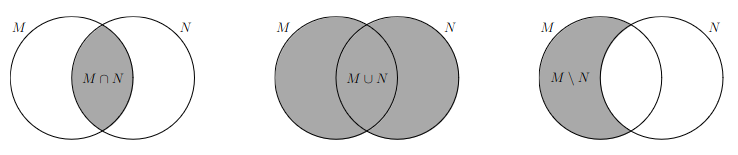
\includegraphics[width=0.75\linewidth]{Mengen.png}
            %    \\
            %\end{figure}\\
            %\begin{figure}[h]
            %    \centering
            %    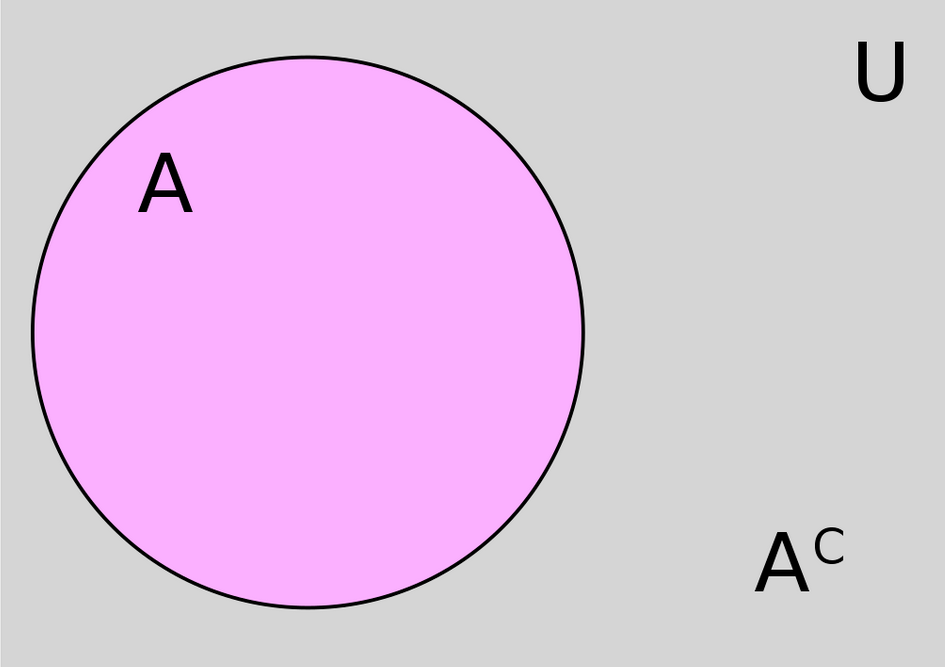
\includegraphics[width=0.25\linewidth]{Screenshot from 2023-10-26 12-00-55.png}
            %\end{figure}
\end{document}
